\chapter{Helios radial line-up passings}

%COFI -- chapter outline and flow integration\\

have a look into Schwenn1984...\\

%motivation
To derive the radial dependence of the solar wind parameters directly, we look at the passings when both Helios spacecraft were radially lined up. In these cases they flew through the same solar wind at different solar distances.\\
(This eliminates the bias of averaging over slow and fast wind streams, like the described model does.)\\
see also \citet{Schwenn1990} p.~156 + p.~122...\\
%Helios line-up mapping techniques -> Schwenn1981 "Two states..." (not findable online after extensive search)

we compare these independently derived radial fit functions to those obtained from the averaging over all solar wind types...\\

%Helios passings, their time and position
There were eight passings when both Helios spacecraft were radially lined-up (see \autoref{fig:Helios12_lineup_positions_v3_pdfcairo_plot}).
\begin{figure}[htb]
	\centering
	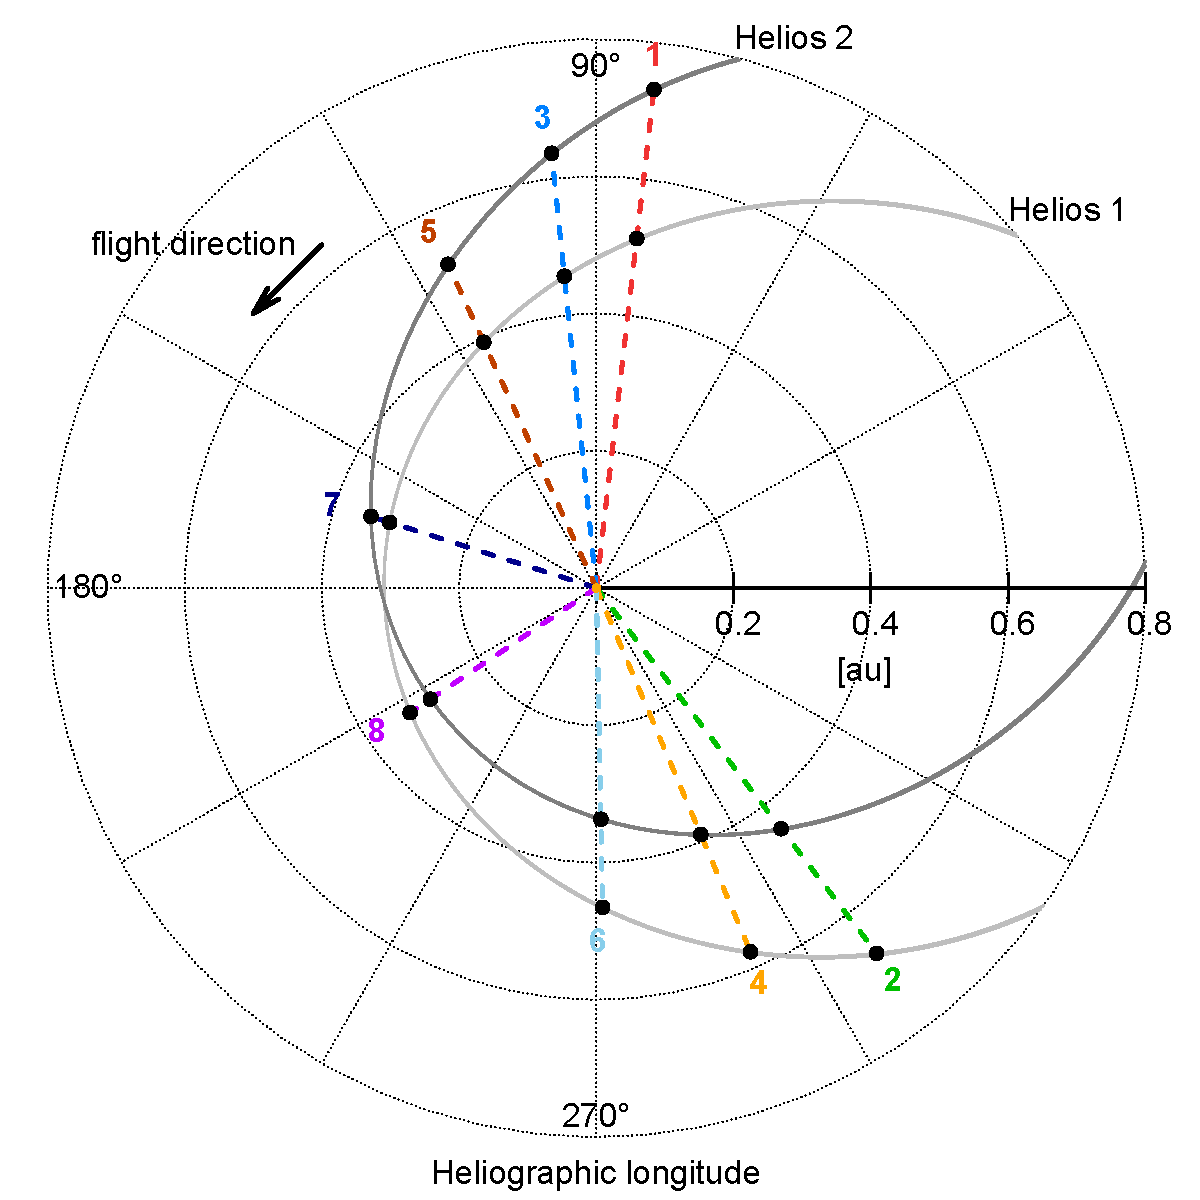
\includegraphics[width=0.6\textwidth]{images/gnuplots/Helios12_lineup_positions_v3_pdfcairo_plot.pdf}
	\caption{Schema of the eight spacecraft line-up positions of both Helios probes on their respective orbits. make B\&W... combine with fig 5.15? calibrate text size}
	\label{fig:Helios12_lineup_positions_v3_pdfcairo_plot}
\end{figure}
These points in time, when both probes had no separation in heliographic longitude, are derived from Helios~1 and Helios~2 daily trajectory data (for the data source see Section~XX). The data is linear interpolated to get an hourly resolution. The resulting points in time together with solar distances are listed in \autoref{tab:lineup_in_longitude}.
\begin{table}[htb]\small
	\centering
	\captionsetup{belowskip=4pt}
	\caption{Times when both Helios probes had no separation in heliographic longitude. Their solar distances (inner spacecraft $r_1$, outer spacecraft $r_2$) were in the range 0.291--0.731~au and the maximal inter-probe radial distance d$r$ was 0.229~au. errors in au...}
	\begin{tabular}{ccccccc}
		\toprule
		\multirow{2}{*}{Passing}	&\multirow{2}{*}{Date}	&\multirow{2}{*}{Time}	&\multirow{2}{*}{Inner s/c}	&$r_1$	&$r_2$	&d$r$\\
			&	&	&	&[au]	&[au]	&[au]\\
		\midrule
		1	&1976-03-09	&00:00	&Helios 1	&0.513	&0.731	&0.219\\
		2	&1976-05-02	&14:00	&Helios 2	&0.442	&0.671	&0.229\\
		3	&1976-09-19	&10:00	&Helios 1	&0.457	&0.637	&0.180\\
		4	&1976-10-31	&11:00	&Helios 2	&0.390	&0.576	&0.186\\
		5	&1977-04-02	&12:00	&Helios 1	&0.394	&0.519	&0.125\\
		6	&1977-04-30	&23:00	&Helios 2	&0.337	&0.465	&0.128\\
		7	&1977-10-18	&06:00	&Helios 1	&0.316	&0.345	&0.029\\
		8	&1977-10-25	&19:00	&Helios 2	&0.291	&0.327	&0.035\\
		\bottomrule
	\end{tabular}
	\label{tab:lineup_in_longitude}
\end{table}
%table data from
%file:///home/raid0/mvenzmer/Desktop/astro70/analyses/Helios12_1h_magswe/Helios12_1h_inline/lineup_periods_v3.txt

%excluding period 7 and 8
The last two passings were merely one week apart and the Helios probes flew almost without radial separation because Helios~2 overtook Helios~1 during its perihelion. As we want to analyze the same solar wind at different solar distances, we exclude the passings 7 and 8 from further analyses.\\


%defining line-up requirements
The passing longitude is not the same as the longitude where the solar wind is detected by both spacecraft consecutively. A passing occurs shortly before the points in time when both spacecraft observe the same solar wind. For the outer probe this point in time is shifted by the solar wind's travel time. The travel time depends on the solar wind's velocity and its distance traveled.\\


%calculation of the offset times
Based on the obtained spacecraft line-up time $t_0$ one can calculate the offset times $t_1$ and $t_2$ when the inner and outer spacecraft pass by the same solar wind (see \autoref{fig:Helios12_lineup_calculation_pdfcairo_plot}). At the solar wind line-up longitude the condition
\begin{align}
	t_2 = t_1 + t_\text{sw} \label{eq:lineup_condition}
\end{align}
holds. As the offset times depend on the solar wind travel time between the probes, we need knowledge of the solar wind velocity $v$ for their calculation: $t_\text{sw} = \text{d}r/v$, with the mean radial separation distance d$r$ between the probes.
\begin{figure}[htb]
	\centering
	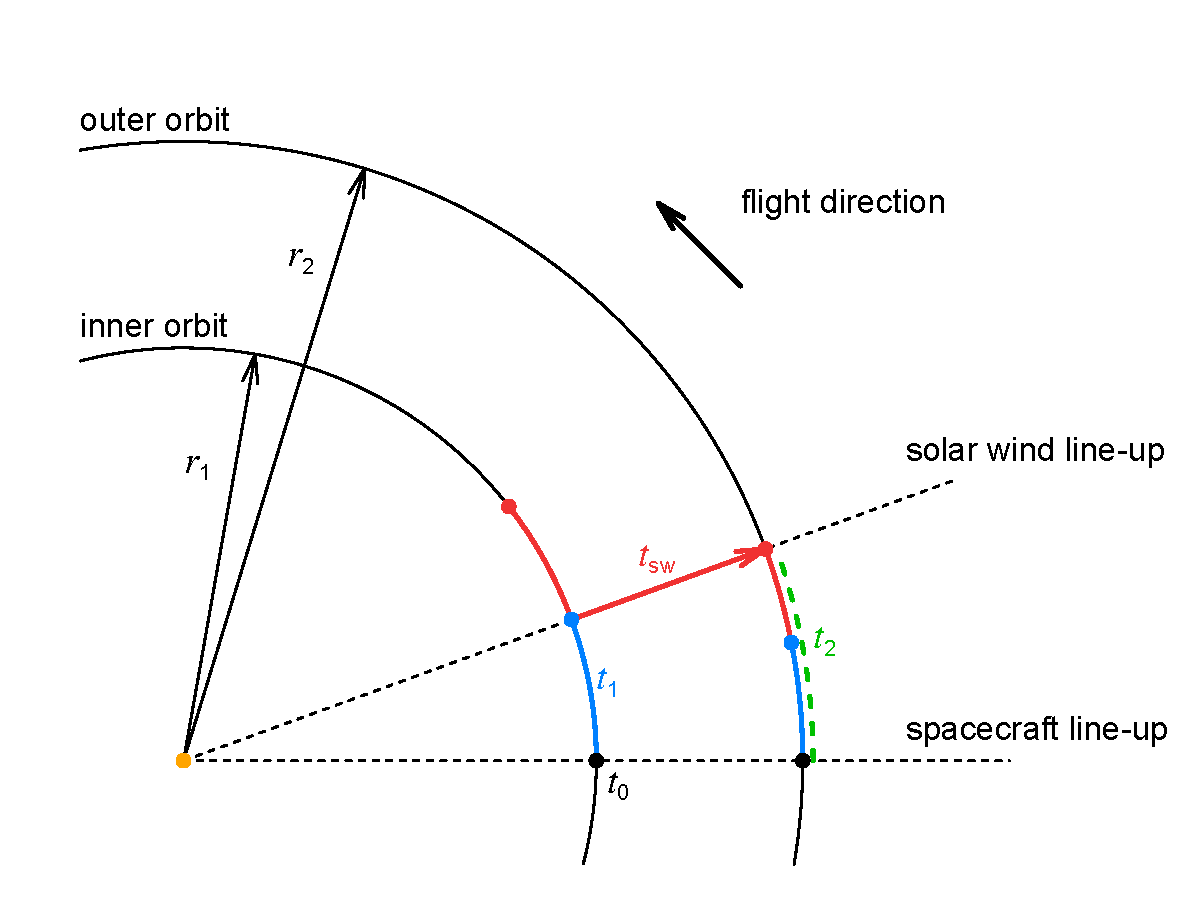
\includegraphics[width=0.5\textwidth]{images/gnuplots/Helios12_lineup_calculation_pdfcairo_plot.pdf}
	\caption{Illustration of the solar wind line-up longitude situation with the spacecraft line-up time $t_0$, the offset times $t_1$, $t_2$ (at which the spacecraft measure the same solar wind) and the solar wind travel time $t_\text{sw}$. combine with fig 5.14?}
	\label{fig:Helios12_lineup_calculation_pdfcairo_plot}
\end{figure}
%/home/raid0/mvenzmer/Desktop/astro70/analyses/Helios12_1h_magswe/Helios12_1h_inline/Helios12_lineup_calculation_pdfcairo_gps.txt

%calculating t_1
For the calculation of $t_1$ we recall the third Kepler law
\begin{align}
	\frac{{T_1}^2}{{T_2}^2} = \frac{{a_1}^3}{{a_2}^3}
\end{align}
with the orbital periods $T_1$, $T_2$ and the semi-major axes $a_1$, $a_2$. The assumption of circular orbits (why? what error size?) leads to
\begin{align}
	\frac{{t_1}^2}{(t_1 + t_\text{sw})^2} &= \frac{{r_1}^3}{{r_2}^3}	\nonumber\\
	\Leftrightarrow\qquad\qquad	t_1 &= t_\text{sw} \left( \left( \frac{r_1}{r_2} \right)^\frac{3}{2} - 1 \right)^{-1} \label{eq:offset_time}
\end{align}
and finally the offset time $t_1$ only depends on the variable solar wind travel time $t_\text{sw}$.\\

%calculating the offset time from the solar wind velocity
Due to uncertainties in the travel time $t_\text{sw}$ (the solar wind speed $v$ is obviously not a constant) the exact calculation of $t_1$ is imprecise. To get a reliable result we perform two iterations calculating the offset time from the average velocity $\bar{v}$ of the surrounding 2-day period. We use the velocity $\bar{v}_0$ around $t_0$ to calculate the offset time $t'_1$ as a first estimate. As the velocity $\bar{v}'_1$ at $t'_1$ is certainly different, we use this velocity to refine the value and obtain $t_1$. Hence deriving the velocity $\bar{v}_1$ enables us to calculate the solar wind travel time $t_\text{sw}$.

%We have to round the offset times and time shift values to full hours, because we use the hourly merged mag and plasma Helios data set (see Section~XX) for the velocity calculation.
The average velocities are obtained from the hourly merged (mag?) and (plasma?) Helios data set (see Section~XX). The resulting offset times and velocities of both iterations together with the travel times are listed in \autoref{tab:offset_times}.
\begin{table}[htb]\small
	\centering
	\captionsetup{belowskip=4pt}
	\caption{The two iterations of the derived offset times and average velocities. The resulting solar wind travel times have durations of 11--28~hours. errors...}
	\begin{tabular}{cccccccc}
		\toprule
		\multirow{2}{*}{Passing}	&\multirow{2}{*}{Inner s/c}	&$v_0$	&$t'_1$	&$v'_1$	&$t_1$	&$v_1$	&$t_\text{sw}$\\
			&	&[km/s]	&[h]	&[km/s]	&[h]	&[km/s]	&[h]\\
		\midrule
		1	&Helios 1	&659.3	&19.6	&656.9	&19.7	&656.9	&13.9\\
		2	&Helios 2	&436.4	&25.1	&370.9	&29.5	&356.7	&26.7\\
		3	&Helios 1	&482.6	&24.0	&444.0	&26.1	&413.8	&18.1\\
		4	&Helios 2	&302.3	&32.2	&279.9	&34.8	&278.3	&27.8\\
		5	&Helios 1	&507.3	&20.0	&474.8	&21.4	&473.5	&11.0\\
		6	&Helios 2	&321.2	&26.6	&392.6	&21.7	&367.8	&14.5\\
		\bottomrule
	\end{tabular}
	\label{tab:offset_times}
\end{table}
%table data from
%file:///home/raid0/mvenzmer/Desktop/astro70/analyses/Helios12_1h_magswe/Helios12_1h_inline/lineup_periods_v3.txt

%introducing the lag time for arbitrary longitude positions
For the solar wind line-up longitude condition~\eqref{eq:lineup_condition} holds. For all other positions the solar wind measured by the inner spacecraft will not arrive the outer orbit position at the same time as the outer spacecraft does (see \autoref{fig:Helios12_lineup_calculation_delay_pdfcairo_plot}).
\begin{figure}[htb]
	\centering
	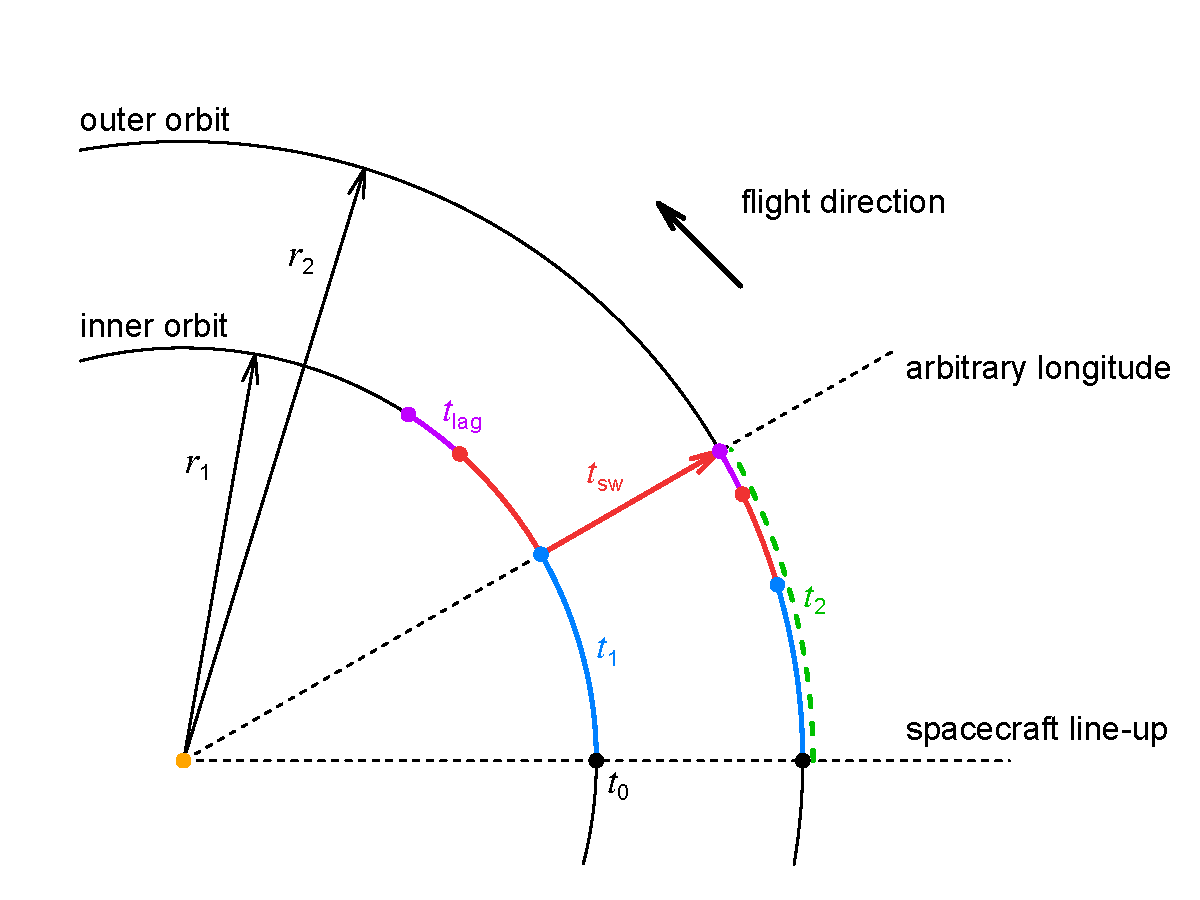
\includegraphics[width=0.5\textwidth]{images/gnuplots/Helios12_lineup_calculation_delay_pdfcairo_plot.pdf}
	\caption{Illustration like \autoref{fig:Helios12_lineup_calculation_pdfcairo_plot} but for arbitrary longitude situations a lag time $t_\text{lag}$ comes into play. merge with fig 5.14?}
	\label{fig:Helios12_lineup_calculation_delay_pdfcairo_plot}
\end{figure}
%/home/raid0/mvenzmer/Desktop/astro70/analyses/Helios12_1h_magswe/Helios12_1h_inline/Helios12_lineup_calculation_delay_pdfcairo_gps.txt

Either the spacecraft (negative lag time) or the solar wind (positive lag time) already have passed this position:
\begin{align}
	t_2 = t_1 + t_\text{sw} + t_\text{lag}. \label{eq:lag_time}
\end{align}
This lag time $t_\text{lag}$ is the time difference at which the solar wind is probed by both spacecraft. At the spacecraft line-up longitude ($t_1 = t_2 = 0$) the lag time equals the solar wind travel time and at the solar wind line-up longitude the lag time is zero.\\

%calculation of the +-24 hour solar wind time span
We choose to look at time periods (instead of points in time) around the offset times to derive average solar wind parameters. This helps reducing the influence of solar wind fluctuations.\\

We define the period duration boundaries as when the lag time $t_\text{lag}$ is in the range $\pm24$~h. For the outer spacecraft these periods are almost twice as long as for the inner spacecraft. The calculated period start and end hours (relative to $t_0$) for both spacecraft are listed in \autoref{tab:period_times_coverage} together with the data coverage of these periods.
\begin{table}[htb]\small
	\centering
	\captionsetup{belowskip=4pt}
	\caption{Derived period start and end hours for both spacecraft in relation to the longitude line-up time $t_0$. The corresponding combined data coverage within that period of the magnetic field, velocity, density and temperature is listed as well. instead duration! errors...}
	\begin{tabular}{cccrrccrrc}
		\toprule
		\multirow{3}{*}{Period}	&	&\multicolumn{4}{c}{Inner spacecraft}	&	&\multicolumn{3}{c}{Outer spacecraft}\\
		\cmidrule{3-6}	\cmidrule{8-10}
			&	&\multirow{2}{*}{s/c}	&Start	&End	&Coverage	&	&Start	&End	&Coverage\\
			&	&	&[h]	&[h]	&[\%]	&	&[h]	&[h]	&[\%]\\
		\midrule
		1	&	&Helios 1	&-14.4	&53.8	&73	&	&-24.6	&91.6	&99\\
		2	&	&Helios 2	&3.1	&58.3	&89	&	&5.8	&109.0	&88\\
		3	&	&Helios 1	&-9.2	&65.1	&16	&	&-15.1	&107.2	&10\\
		4	&	&Helios 2	&4.8	&65.2	&59	&	&8.5	&117.0	&87\\
		5	&	&Helios 1	&-25.5	&68.3	&89	&	&-38.5	&103.3	&88\\
		6	&	&Helios 2	&-15.3	&61.7	&93	&	&-24.8	&100.1	&92\\
		\bottomrule
	\end{tabular}
	\label{tab:period_times_coverage}
\end{table}
% %table data from
% %file:///home/raid0/mvenzmer/Desktop/astro70/analyses/Helios12_1h_magswe/Helios12_1h_inline/lineup_periods_v3.txt

%excluding period 3
For period~3 the combined data coverage of the four solar wind parameters is only 16~\% (Helios~1) and 10~\% (Helios~2) respectively. We consider this as insufficient for the continuing analysis and therefore also omit period~3.\\

The five remaining periods are marked in \autoref{fig:Helios12_lineup_period_positions_v3_pdfcairo_plot}.
\begin{figure}[htb]
	\centering
	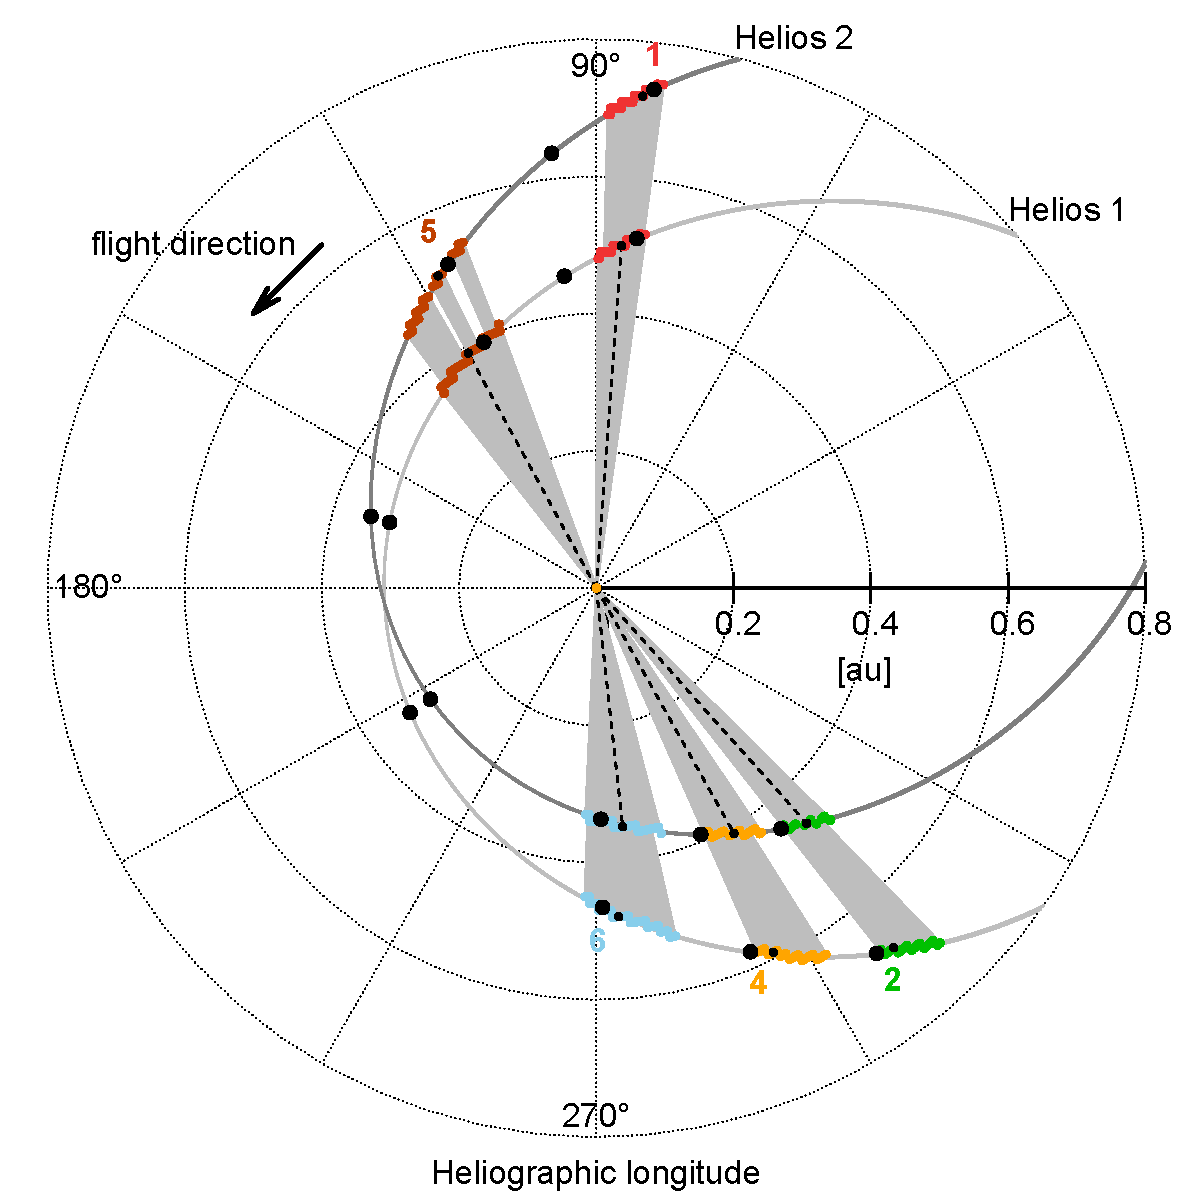
\includegraphics[width=0.6\textwidth]{images/gnuplots/Helios12_lineup_period_positions_v3_pdfcairo_plot.pdf}
	\caption{Scheme of the line-up periods of both Helios spacecraft on their respective orbits. The corresponding orbit sections which we consider in our analysis are marked in color. These sections span the positions where both spacecraft observed the same solar wind with a maximal lag time of $\pm24$~hours. bw figure?? dotted lines?}
	\label{fig:Helios12_lineup_period_positions_v3_pdfcairo_plot}
\end{figure}

%average values
The average values of the four parameters magnetic field $B$, velocity $v$, density $n$ and temperature $T$ are listed in \autoref{tab:period_means}.
\begin{table}[htb]\small
	\centering
	\captionsetup{belowskip=4pt}
	\caption{Average values of the four solar wind parameters magnetic field, velocity, density and temperature for the individual periods and spacecraft. errors...}
	\begin{tabular}{cccrrrrcrrrr}
		\toprule
		\multirow{3}{*}{Period}	&	&\multicolumn{5}{c}{Inner spacecraft}	&	&\multicolumn{4}{c}{Outer spacecraft}\\
		\cmidrule{3-7}	\cmidrule{9-12}
			&	&\multirow{2}{*}{s/c}	&\multicolumn{1}{c}{$B$}	&\multicolumn{1}{c}{$v$}	&\multicolumn{1}{c}{$n$}	&\multicolumn{1}{c}{$T$}	&	&$B$	&$v$	&$n$	&$T$\\
			&	&	&\multicolumn{1}{c}{[nT]}	&\multicolumn{1}{c}{[km/s]}	&\multicolumn{1}{c}{[cm$^{-3}$]}	&\multicolumn{1}{c}{[K]}	&	&[nT]	&[km/s]	&[cm$^{-3}$]	&[K]\\
		\midrule
		1	&	&Helios 1	&17.04	&646.4	&12.0	&367\,300	&	&8.93	&602.8	&6.7	&244\,000\\
		2	&	&Helios 2	&15.77	&356.4	&38.8	&122\,400	&	&12.05	&390.2	&17.7	&117\,200\\
		4	&	&Helios 2	&15.18	&281.3	&108.0	&46\,000	&	&10.64	&298.6	&46.1	&30\,400\\
		5	&	&Helios 1	&28.80	&521.3	&45.9	&337\,800	&	&18.73	&530.3	&24.4	&282\,000\\
		6	&	&Helios 2	&29.57	&402.4	&82.5	&271\,900	&	&14.71	&432.6	&35.7	&199\,100\\
		\bottomrule
	\end{tabular}
	\label{tab:period_means}
\end{table}
%table data from
%file:///home/raid0/mvenzmer/Desktop/astro70/analyses/Helios12_1h_magswe/Helios12_1h_inline/lineup_periods_v3.txt

%solar wind feature match
If we compare both, the inner solar wind sections together with their outer counterparts, they indeed appear to have a similar shape apart from the time shift (see \autoref{fig:Helios12_lineup_period_1_7d_v3_plot}) (name definite features...). This confirmes that they indeed are parts of the same solar wind structures.\\
maybe figures of all into Appendix?...\\
\begin{figure}[htb]
	\centering
	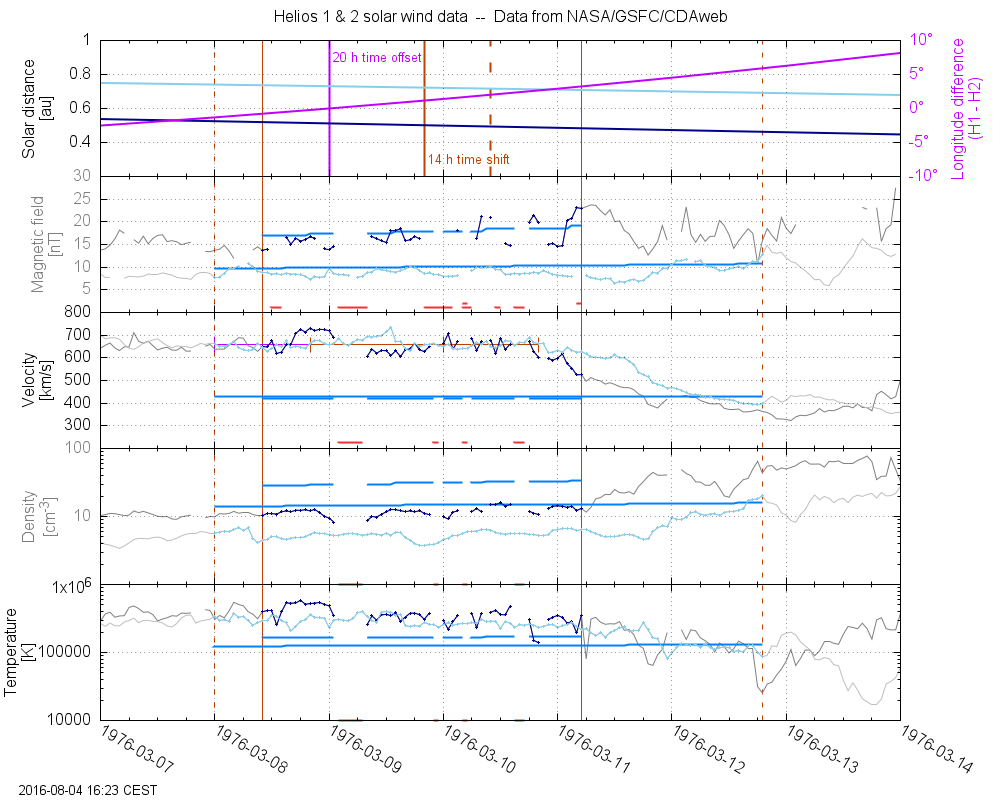
\includegraphics[width=0.5\textwidth]{images/gnuplots/Helios12_lineup_period_1_7d_v3_plot.png}
	\caption{Measured solar wind parameters $B$, $v$, $n$, and $T$ of both spacecraft in the period~1. Also plotted is the spacecraft's separation in heliographic longitude. offset time, time shift; expected value from the radial sw model... remove date... remove solar distance... adjust text size...}
	\label{fig:Helios12_lineup_period_1_7d_v3_plot}
\end{figure}


%solar wind types
the comparison to the sw model's mean value at the individual distances lets us classify the solar wind types...
\begin{description*}
	\item[Period 1]	HSS
	\item[Period 2]	medium--LSS
	\item[Period 4]	LSS
	\item[Period 5]	medium--HSS
	\item[Period 6]	LSS--HSS
\end{description*}

%...forward- and back-matching data gaps results in worse data coverage!

%fit function parameters
We obtained the mean parameter values for the inner and outer solar wind sections. As with the overall radial dependency before, these two points are fitted to the exponential regression fit function $X(r) = X_0\,r^{c_X}$ (see Section~XX. The resulting fit coefficients for each period are listed in \autoref{tab:lineup_fit_functions}.\\
why is it better to fit the period's mean values than the whole period?...\\
we fit the periods' mean value rather than the whole periods, because...\\

\begin{table}[htb]\small
	\centering
	\captionsetup{belowskip=4pt}
	\caption{Radial fit functions $B(r)$, $v(r)$, $n(r)$ and $T(r)$ for each period. or only the variables into table? error sizes...}
	\begin{tabular}{cgggg}
		\toprule
		\multirow{2}{*}{Period}	&B(r) =,B_0~r^{c_B}	&v(r) =,v_0~r^{c_v}	&n(r) =,n_0~r^{c_n}	&T(r) =,T_0~r^{c_T}\\
			&\text{[nT]},	&\text{[km/s]},	&\text{[cm$^{-3}$]},	&\text{[K]},\\
		\midrule
		1	&4.88,r^{-1.815}	&564.7,r^{-0.196}	&3.9,r^{-1.647}	&166\,500,r^{-1.148}\\
		2	&9.50,r^{-0.654}	&442.6,r^{0.220}	&8.9,r^{-1.902}	&112\,800,r^{-0.106}\\
		4	&6.79,r^{-0.900}	&322.0,r^{0.151}	&15.7,r^{-2.155}	&18\,000,r^{-1.047}\\
		5	&5.99,r^{-1.649}	&554.8,r^{0.065}	&4.6,r^{-2.423}	&174\,700,r^{-0.692}\\
		6	&3.22,r^{-2.108}	&506.5,r^{0.219}	&5.7,r^{-2.533}	&101\,000,r^{-0.941}\\
		\midrule
		weigthed by duration mean functions\\
		\midrule
		mean of sw model (update)	&6.078,r^{-1.563}	&435.5,r^{0.04955}	&7.613,r^{-2.032}	&97\,050,r^{-0.8002}\\
		\bottomrule
	\end{tabular}
	\label{tab:lineup_fit_functions}
\end{table}
%table data from
%file:///home/raid0/mvenzmer/Desktop/astro70/analyses/Helios12_1h_magswe/Helios12_1h_inline/lineup_periods_v3.txt

%interpretation
The fit curves show noticeable deviations from the model's mean fit (see \autoref{fig:Helios12_lineup_fit_Bmean_v3_final_plot}). maybe 4-panel figure?; maybe figures of all into Appendix?\\
\begin{figure}[htb]
	\centering
	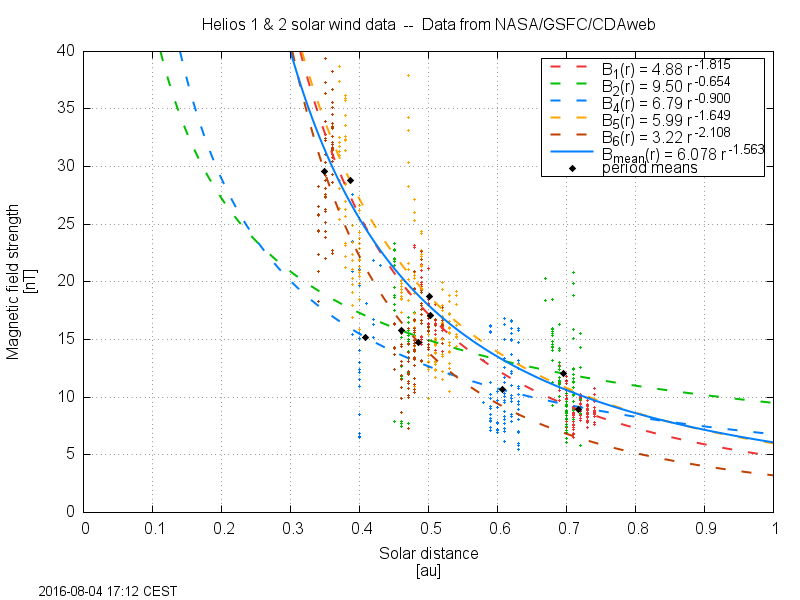
\includegraphics[width=0.5\textwidth]{images/gnuplots/Helios12_lineup_fit_Bmean_v3_final_plot.png}
	\caption{Fit curves of the radial magnetic field. The fits are based on the mean values (meanr,meanB; black points) of the line-up periods. build pdf figure... remove date... adjust text size... 4-figure?}
	\label{fig:Helios12_lineup_fit_Bmean_v3_final_plot}
\end{figure}
The observed deviations are as expected from these types of solar wind. ...are they? analyze each in detail...\\
argue from sw type; slow, medium and fast type; check their position relative to the mean curve...\\

%what we have learned
results:\\
features of calculated line-up periods match.\\
their derived fit functions scatter within (acceptable?) margin around model's radial mean, backing its applicability.\\


